
%----------------------------------------------------------------------------------------
%	PACKAGES AND OTHER DOCUMENT CONFIGURATIONS
%----------------------------------------------------------------------------------------

\documentclass[a4paper]{article}

\usepackage{amsmath}

\usepackage{amssymb}

\usepackage{mhchem}

\usepackage{gensymb}

%\usepackage[super]{natbib}

\usepackage[T1]{fontenc} % Use 8-bit encoding that has 256 glyphs

\usepackage{lmodern}

\usepackage[hyphenbreaks]{breakurl}

\usepackage[hyphens]{url}

%\usepackage[super,sort&compress]{natbib}
%\usepackage{natbib}
%\setlength{\bibsep}{0.0pt}

\usepackage{subcaption}

\usepackage{graphicx}

\linespread{1.05} % Line spacing - Palatino needs more space between lines
\usepackage{microtype} % Slightly tweak font spacing for aesthetics

\usepackage[spanish]{babel} % Language hyphenation and typographical rules

\usepackage[numbib,notlof,notlot,nottoc]{tocbibind} % Shows bibliography as a section

\usepackage[hmarginratio=1:1,top=32mm,columnsep=20pt]{geometry} % Document margins

\usepackage[section]{placeins}

\usepackage{float}

\usepackage{booktabs} % Horizontal rules in tables

\usepackage{enumitem} % Customized lists


\usepackage{abstract} % Allows abstract customization

\renewcommand{\abstractnamefont}{\normalfont\bfseries} % Set the "Abstract" text to bold

\usepackage{fancyhdr} % Headers and footers
\pagestyle{fancy} % All pages have headers and footers
\fancyhead{} % Blank out the default header
\fancyfoot{} % Blank out the default footer
\fancyhead[C]{Apuntes y ejercicios resueltos de Estructura de la Materia 2} % Custom header text
\fancyfoot[C]{\thepage} % Custom footer text

\usepackage{titling} % Customizing the title section

\usepackage{hyperref} % For hyperlinks in the PDF

%----------------------------------------------------------------------------------------
%	TITLE SECTION
%----------------------------------------------------------------------------------------

\setlength{\droptitle}{-4\baselineskip} % Move the title up

\pretitle{\begin{center}\LARGE\bfseries} % Article title formatting
\posttitle{\end{center}} % Article title closing formatting
\title{Estructura de la Materia 2} % Article title
\author{%
\textsc{Ignacio Poggi} \\[1ex] % Your name
\normalsize \href{mailto:ignaciop.3@gmail.com}{ignaciop.3@gmail.com} % Your email address
}

\date{\today} % Leave empty to omit a date
\renewcommand{\maketitlehookd}{%
\begin{abstract}
Apuntes y ejercicios resueltos de Estructura de la Materia 2 (2º cuatrimestre 2022).
\end{abstract}
}

%----------------------------------------------------------------------------------------

\begin{document}
\maketitle

% Print the title
%----------------------------------------------------------------------------------------


\tableofcontents
% Table of contents

%----------------------------------------------------------------------------------------
%	ARTICLE CONTENTS
%----------------------------------------------------------------------------------------

\section{Gu\'ia 1: Redes Cristalinas y Espacio Rec\'iproco}

\subsection{}

\begin{itemize}
\item En este \'item nos piden describir una estructura c\'ubica centrada en la base (SC con puntos adicionales en las caras horizontales de la celda).

\begin{figure}[H]
  \centering
  \begin{subfigure}[b]{0.4\linewidth}
    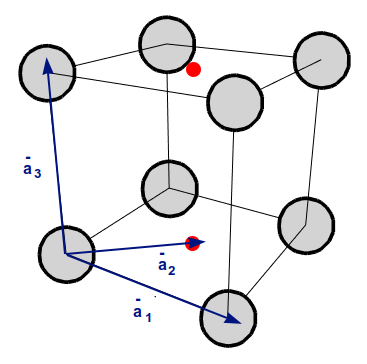
\includegraphics[width=\linewidth]{cubo3d_ej1.png}
     \caption{Red c\'ubica centrada en la base con una posible elecci\'on de vectores primitivos.}
  \end{subfigure}
  \begin{subfigure}[b]{0.4\linewidth}
    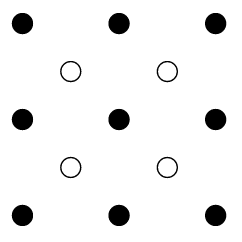
\includegraphics[width=\linewidth]{red_cubica.png}
    \caption{Vista cenital de la red peri\'odica.}
  \end{subfigure}
  \label{fig:cubo3d_ej1}
\end{figure}

Esta red puede pensarse como suma de planos con dos redes SC en dos dimensiones superpuestas, por lo tanto, es red de Bravais (de ahora en adelante, RB).

Una posible elecci\'on de vectores primitivos es la siguiente:

$$\begin{cases}
\vec{a}_{1} = a\hat{x} \\
\vec{a}_{2} = \frac{a}{2}(\hat{x} + \hat{y}) \\
\vec{a}_{3} = a\hat{z}
\end{cases}$$

\item Para la c\'ubica centrada en los lados (SC con puntos adicionales en las caras verticales de la celda), es an\'alogo al caso a), describiendo a los vectores primitivos de la siguiente manera:

\begin{figure}[H]
  \centering
  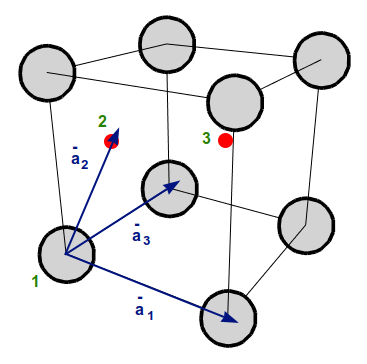
\includegraphics[width=0.5\linewidth,height=0.5\linewidth]{cubo3d_ej2.png}
  \caption{Red c\'ubica centrada en la base con una posible elecci\'on de vectores primitivos.}
  \label{fig:cubo3d_ej2}
\end{figure}

Observamos que no es una RB (como vemos en la figura (\ref{fig:cubo3d_ej2}) en color verde, desde el punto 2, vemos al punto 3; pero desde \'este no llegamos a 1). Podemos describir la red como una \textit{SC + base}:

$$base = \{ \vec{0}, \frac{a}{2}(\hat{z} + \hat{y}), \frac{a}{2}(\hat{x} + \hat{z})\}$$

\item Para la red c\'ubica centrada en las aristas, tenemos el mismo problema que la anterior (desde el punto 2 tengo al punto vecino 3; que no se ve desde 1 $\Rightarrow$ no es RB.

\begin{figure}[H]
  \centering
  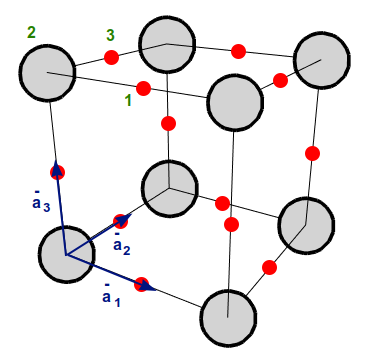
\includegraphics[width=0.5\linewidth,height=0.5\linewidth]{cubo3d_ej3.png}
  \caption{Red c\'ubica centrada en la base con una posible elecci\'on de vectores primitivos.}
  \label{fig:cubo3d_ej3}
\end{figure}

La describimos as\'i:

$$SC + base = SC + \{ \vec{0}, \frac{a}{2}\hat{x}, \frac{a}{2}\hat{y}, \frac{a}{2}\hat{z}\}$$

\end{itemize}

\subsection{}

\textbf{Red BCC (Body Centered Cube):}

\begin{figure}[H]
  \centering
  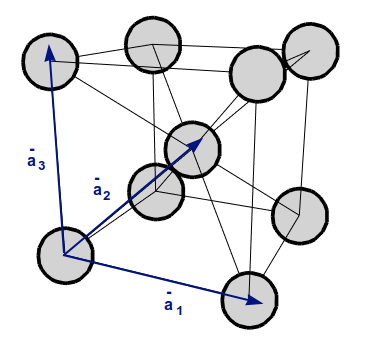
\includegraphics[width=0.5\linewidth,height=0.5\linewidth]{bcc.png}
  \caption{Red BCC con una posible elecci\'on de vectores primitivos.}
  \label{fig:bcc}
\end{figure}

Como vemos en la figura (\ref{fig:bcc}), uno de los posibles conjuntos de vectores primitivos para esta red es:

$$\begin{cases}
\vec{a}_{1} = a\hat{x} \\
\vec{a}_{2} = \frac{a}{2}(\hat{x} + \hat{y} + \hat{z}) \\
\vec{a}_{3} = a\hat{z}
\end{cases}$$

Otra elecci\'on:

$$\begin{cases}
\vec{a}_{1}' = a(\hat{x} + \hat{y}) \\
\vec{a}_{2}' = \frac{a}{2}(\hat{x} + \hat{y} + \hat{z}) \\
\vec{a}_{3}' = a(\hat{y} + \hat{z})
\end{cases}$$

Para hallar el volumen de la celda unidad, utilizamos la relaci\'on:

\begin{equation}
\label{eq:vol_celda_unidad}
V = | \vec{a}_{1} \cdot (\vec{a}_{2} \times \vec{a}_{3})|
\end{equation}

donde los $\vec{a}_{i}$ son los vectores primitivos. Entonces:

$$ \vec{a}_{2} \times \vec{a}_{3} = \begin{vmatrix}
\frac{a}{2} & \frac{a}{2} & \frac{a}{2} \\ 
0 & 0 & a
\end{vmatrix}  = (\frac{a^{2}}{2}, -\frac{a^{2}}{2}, 0) = \frac{a^{2}}{2}(\hat{x} - \hat{y})$$

$$ \Rightarrow \vec{a}_{1} \cdot (\vec{a}_{2} \times \vec{a}_{3}) = (a, 0, 0) \cdot (\frac{a^{2}}{2}, -\frac{a^{2}}{2}, 0) = \frac{a^{3}}{2}$$

$$ \Rightarrow V_{BCC} = | \vec{a}_{1} \cdot (\vec{a}_{2} \times \vec{a}_{3})| = |\frac{a^{3}}{2}| = \frac{a^{3}}{2}$$

Con la otra elecci\'on de vectores primitivos $\vec{a}_{i}'$, obtenemos el mismo resultado.\\

\textbf{Red FCC (Face Centered Cube):}

\begin{figure}[H]
  \centering
  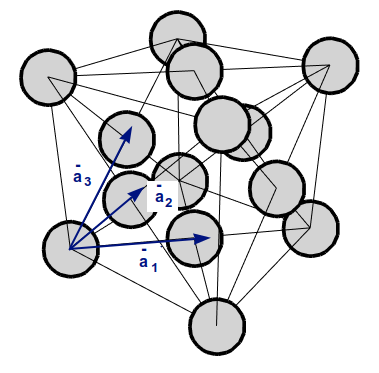
\includegraphics[width=0.5\linewidth,height=0.5\linewidth]{fcc.png}
  \caption{Red FCC con una posible elecci\'on de vectores primitivos.}
  \label{fig:fcc}
\end{figure}

Observamos en la a figura (\ref{fig:fcc}), los vectores primitivos para esta red:

$$\begin{cases}
\vec{a}_{1} = \frac{a}{2}(\hat{x} + \hat{y}) \\
\vec{a}_{2} = \frac{a}{2}(\hat{x} + \hat{z}) \\
\vec{a}_{3} = \frac{a}{2}(\hat{y} + \hat{z})
\end{cases}$$

Una elecci\'on m\'as turbia ser\'ia:

$$\begin{cases}
\vec{a}_{1}' = \frac{a}{2}(\hat{x} + \hat{y}) - a\hat{z} \\
\vec{a}_{2}' = a\hat{x} + \frac{a}{2}(\hat{y} + \hat{z}) \\
\vec{a}_{3}' = a\hat{z}
\end{cases}$$

Luego:

$$ \vec{a}_{2} \times \vec{a}_{3} = \begin{vmatrix}
\frac{a}{2} & 0 & \frac{a}{2} \\ 
0 & \frac{a}{2} & \frac{a}{2}
\end{vmatrix}  = (-\frac{a^{2}}{4}, -\frac{a^{2}}{4}, \frac{a^{2}}{4}) = \frac{a^{2}}{4}(- \hat{x} - \hat{y} + \hat{z})$$

$$ \Rightarrow \vec{a}_{1} \cdot (\vec{a}_{2} \times \vec{a}_{3}) = (\frac{a}{2}, \frac{a}{2}, 0) \cdot (-\frac{a^{2}}{4}, -\frac{a^{2}}{4}, \frac{a^{2}}{4}) = -\frac{a^{3}}{4}$$

Aplicamos (\ref{eq:vol_celda_unidad}) para hallar el volumen de esta celda:

$$ \Rightarrow V_{FCC} = | \vec{a}_{1} \cdot (\vec{a}_{2} \times \vec{a}_{3})| = |-\frac{a^{3}}{4}| = \frac{a^{3}}{4}$$

\subsection{}

Los primeros vecinos, por definici\'on, son todos aquellos que est\'an a distancia m\'inima de un elemento de la red. Se denomina \textbf{n\'umero de coordinaci\'on} al numero total de \'estos.\\

Los segundos y terceros vecinos son los que le siguen en distancia, respectivamente.\\

\textbf{Red c\'ubica simple:}\\

Para identificar m\'as f\'acilmente a los vecinos, ve\'amosla en 2D (teniendo en cuenta que la figura se repite en $\pm \hat{z}$, hac\'ia afuera/dentro de la hoja):

\begin{figure}[H]
  \centering
  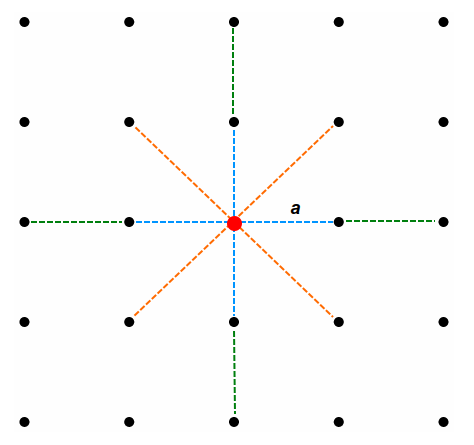
\includegraphics[width=0.5\linewidth,height=0.5\linewidth]{red2d_sc.png}
  \caption{Plano $xy$ de la red c\'ubica. Las l\'ineas azules marcan la distancia a primeros vecinos, las naranjas a segundos vecinos; y las verdes a terceros vecinos. El par\'ametro de red es $a$.}
  \label{fig:red2d_sc}
\end{figure}
 
Simplemente contamos los puntos y calculamos las respectivas distancias al elemento elegido (rojo):

\begin{center}
\# primeros vecinos = 6 (4 en el plano $xy$, 1 en $+\hat{z}$ y 1 en $-\hat{z}$) $\Rightarrow d = a$ \\
\# segundos vecinos = 12 (4 en el plano $xy$, 4 en $+\hat{z}$ y 4 en $-\hat{z}$) $\Rightarrow d = \sqrt{2a}$ \\
\# terceros vecinos = 8 (4 en $+\hat{z}$ y 4 en $-\hat{z}$) $\Rightarrow d = \sqrt{3a}$ \\
\end{center}

En 3D:

\begin{figure}[H]
  \centering
  \begin{subfigure}[b]{0.4\linewidth}
    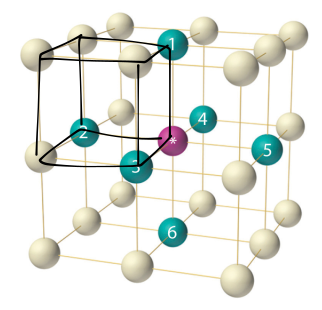
\includegraphics[width=\linewidth]{red3d_sc0.png}
     \caption{Primeros vecinos en color verde.}
  \end{subfigure}
  \begin{subfigure}[b]{0.4\linewidth}
    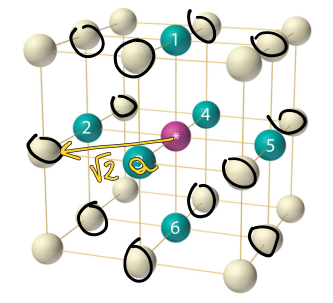
\includegraphics[width=\linewidth]{red3d_sc1.png}
    \caption{Segundos vecinos marcados en negro.}
  \end{subfigure}
  \begin{subfigure}[b]{0.4\linewidth}
    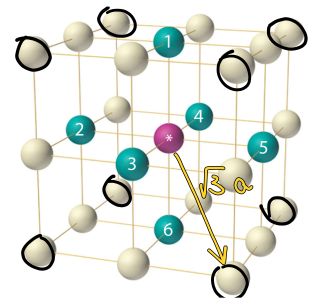
\includegraphics[width=\linewidth]{red3d_sc2.png}
    \caption{Terceros vecinos marcados en negro.}
  \end{subfigure}
  \caption{Primeros, segundos y terceros vecinos de una red SC tridimensional.}
  \label{fig:red3d_Sc}
\end{figure}

\textbf{Red BCC:}\\

\begin{figure}[H]
  \centering
  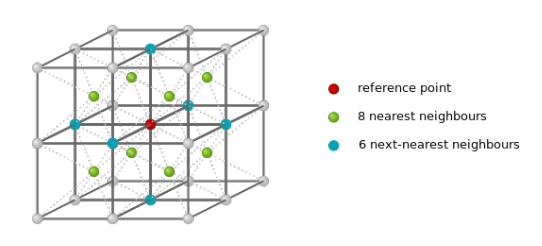
\includegraphics[width=0.7\linewidth,height=0.3\linewidth]{red3d_bcc.png}
  \caption{Primeros, segundos y terceros vecinos de una red BCC tridimensional.}
  \label{fig:red3d_bcc}
\end{figure}

\textbf{Red FCC:}\\

\begin{figure}[H]
  \centering
  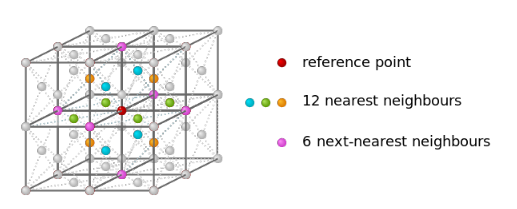
\includegraphics[width=0.7\linewidth,height=0.3\linewidth]{red3d_fcc.png}
  \caption{Primeros, segundos y terceros vecinos de una red FCC tridimensional.}
  \label{fig:red3d_fcc}
\end{figure}

\subsection{}

La fracci\'on de empaquetamiento es la relaci \'on entre el volumen de las esferas (\'atomos) y el volumen de la celda unidad:

\begin{equation}
\label{eq:empaq}
\rho_{X} = \frac{\frac{4}{3}\pi r^{3}}{V_{X}}
\end{equation}

donde

$$r = \frac{d_{1^{o} vecinos}}{2}$$

En la siguiente figura se observan las distribuciones aproximadas para cada red pedida:

\begin{figure}[H]
  \centering
  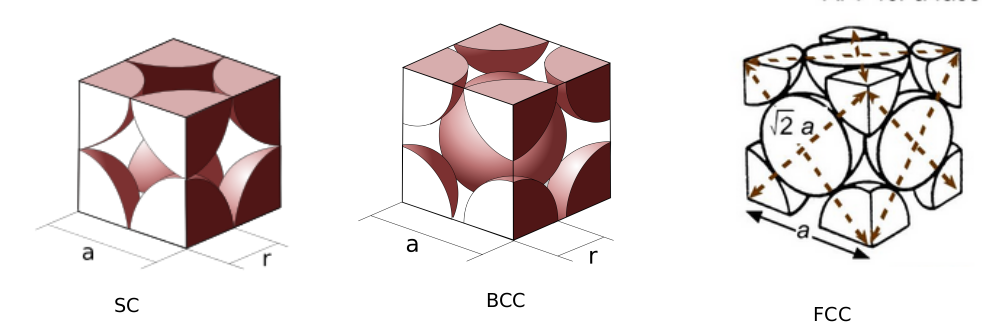
\includegraphics[width=0.9\linewidth,height=0.5\linewidth]{empaq.png}
  \caption{Empaquetamientos de las redes SC, BCC y FCC.}
  \label{fig:empaq}
\end{figure}

Aplicamos la ecuaci\'on (\ref{eq:empaq}) a cada red, con los datos de las distancias a primeros vecinos y volumen de cada celda unidad obtenidos en el ejercicio anterior, entonces:

$$ \rho_{SC} = \frac{\frac{4}{3}\pi r^{3}}{V_{SC}} = \frac{\frac{4}{3}\pi (\frac{a}{2})^{3}}{a^{3}} = \frac{\pi}{6} \approx 0.52$$

Esto quiere decir que, aproximadamente, el 52\% de la celda unidad SC est\'a ocupada por \'atomos.

$$ \rho_{BCC} = \frac{\frac{4}{3}\pi r^{3}}{V_{BCC}} = \frac{\frac{4}{3}\pi (\frac{\sqrt{3}}{4}a)^{3}}{\frac{a^{3}}{2}} = \frac{\sqrt{3}}{8}\pi \approx 0.68$$

$$ \rho_{FCC} = \frac{\frac{4}{3}\pi r^{3}}{V_{FCC}} = \frac{\frac{4}{3}\pi (\frac{\sqrt{3}}{2}a)^{3}}{\frac{a^{3}}{4}} = \frac{\sqrt{2}}{6}\pi \approx 0.74$$

Para la red diamante, veamos un esquema para orientarnos un poco mejor:

\begin{figure}[H]
  \centering
  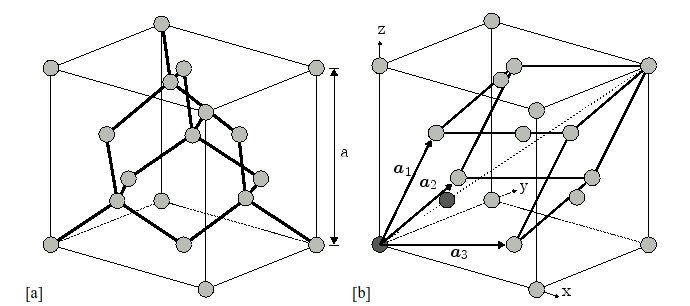
\includegraphics[width=0.9\linewidth,height=0.5\linewidth]{red3d_diamante.png}
  \caption{(a) Celda unidad de la estructura de diamante. (b) Se resaltan los vectores primitivos de una FCC, m\'as los dos \'atomos que conforman la base.}
  \label{fig:red3d_diamante}
\end{figure}

Esta red puede pensarse como dos FCC intercaladas, desplazadas una de la otra sobre la diagonal en $\frac{a}{4}(1, 1, 1)$.\\

Podemos hacer la siguiente elecci\'on para los vectores primitivos:

$$\begin{cases}
\vec{a}_{1} = \frac{a}{2}(\hat{y} + \hat{z}) \\
\vec{a}_{2} = \frac{a}{2}(\hat{x} + \hat{z}) \\
\vec{a}_{3} = \frac{a}{2}(\hat{x} + \hat{y})
\end{cases}$$

Entonces:

$$ Diamante = FCC + \{ \vec{0}, \frac{a}{4}(\hat{x} + \hat{y} + \hat{z})\}$$

Finalmente, calculemos su fracci\'on de empaquetamiento:

$$ \rho_{DIAMANTE} = \frac{\frac{4}{3}\pi r^{3}}{V_{DIAMANTE}} = \frac{\frac{4}{3}\pi (\frac{\sqrt{3}}{8}a)^{3}}{\frac{a^{3}}{4}} = \frac{\sqrt{3}^{3}}{96}\pi \approx 0.17$$

\subsection{}

La estructura subyacente a una HCP (Hexagonal Closed Packed) es una RB hexagonal simple; conformada por varias redes triangulares apiladas. La direcci\'on de apilamiento (usualmente dada por el vector primitivo $\vec{a}_{3}$) se conoce como \textbf{\textit{eje c}}. Sus vectores primitivos son:

$$\begin{cases}
\vec{a}_{1} = a\hat{x} \\
\vec{a}_{2} = \frac{a}{2}\hat{x} + \frac{\sqrt{3}}{2}a\hat{y} \\
\vec{a}_{3} = c\hat{z}
\end{cases}$$

\begin{figure}[H]
  \centering
  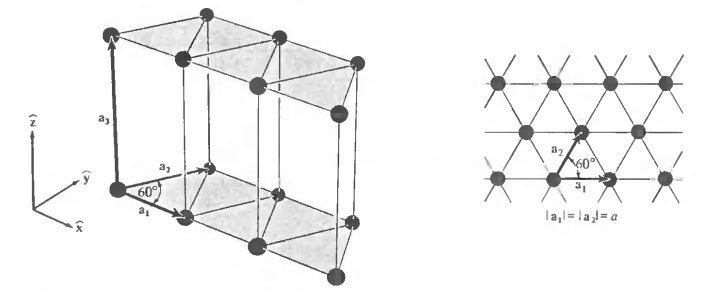
\includegraphics[width=0.9\linewidth,height=0.4\linewidth]{red3d_triangular.png}
  \caption{Red hexagonal simple. Los primeros dos vectores generan la red triangular en el plano $xy$, el tercero lo apila a una distancia $c$.}
  \label{fig:red3d_triangular}
\end{figure}

La red HCP consiste en dos redes hexagonales simples intercaladas, desplazadas una de otra por $\frac{\vec{a}_{1}}{3} + \frac{\vec{a}_{2}}{3} + \frac{\vec{a}_{3}}{2}$, como muestra la siguiente figura:

\begin{figure}[H]
  \centering
  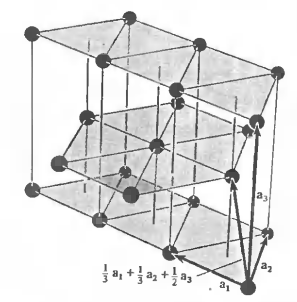
\includegraphics[width=0.5\linewidth,height=0.5\linewidth]{red3d_hcp.png}
  \caption{Red HCP}
  \label{fig:red3d_hcp}
\end{figure}

Sus vectores primitivos son:

$$\begin{cases}
\vec{a}_{1} = \frac{a}{2}\hat{x} - \frac{\sqrt{3}}{2}a\hat{y} \\
\vec{a}_{2} = \frac{a}{2}\hat{x} + \frac{\sqrt{3}}{2}a\hat{y} \\
\vec{a}_{3} = c\hat{z}
\end{cases}$$


Finalmente, calculemos cual es el valor $\frac{c}{a}$ para una red HCP ideal. En la siguiente figura, observamos con detalle una parte de la red para facilitar el c\'alculo:

\begin{figure}[H]
  \centering
  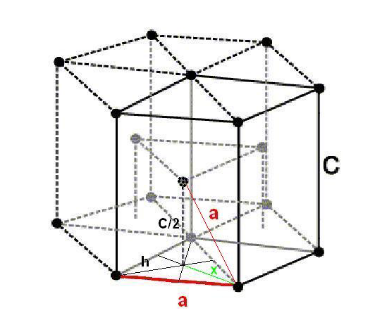
\includegraphics[width=0.5\linewidth,height=0.4\linewidth]{red3d_hcp_r.png}
  \caption{Detalle de una zona de la red HCP.}
  \label{fig:red3d_hcp_r}
\end{figure}

Aqu\'i, $h$ es la altura del tri\'angulo equilatero de lado $a$ (par\'ametro de red). Luego, tenemos la distancia $\frac{c}{2}$, desde el centro de dicho tri\'angulo hasta uno de los puntos de la red triangular intercalada (detalle en figura (\ref{fig:red3d_hcp})). Por \'ultimo, $x$ es la distancia entre uno de los \'atomos de la red tri\'angular hasta el centro del mismo. Entonces:

$$h = \sqrt{a^{2} + \bigg(\frac{a}{2}\bigg)^{2}} = a\sqrt{1 - \frac{1}{4}} = \sqrt{\frac{3}{4}}a$$

$$x = \frac{2}{3}h = \frac{2}{3}\sqrt{\frac{3}{4}}a = \frac{a}{\sqrt{3}}$$

$$\Rightarrow \frac{c}{2} = \sqrt{a^{2} - x^{2}} = \sqrt{a^{2} - \frac{a^{2}}{3}} = \sqrt{\frac{2}{3}}a$$

$$\Rightarrow \frac{c}{a} = \sqrt{\frac{8}{3}} \approx 1.63$$

Obtenemos un valor muy cercano a las estructuras del Mg y Nd.\\

\begin{figure}[H]
  \centering
  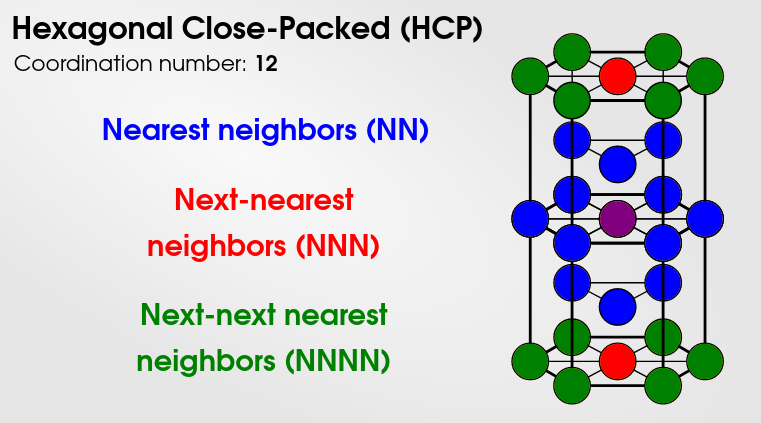
\includegraphics[width=0.5\linewidth,height=0.3\linewidth]{red3d_hcp_n.png}
  \caption{Esquema de la red HCP a primeros, segundos y terceros vecinos.}
  \label{fig:red3d_hcp_n}
\end{figure}

En el esquema anterior, se muestran los primeros vecinos de la red HCP. En el plano del \'atomo de referencia (violeta), tenemos 6 primeros vecinos. Los \'atomos azules tambi\'en son primeros vecinos, que pertenecen a las redes hexagonales intercaladas en $\pm \frac{c}{2}$, d\'andonos un total de \textbf{12 primeros vecinos}. Luego, hay \textbf{2 segundos vecinos}, marcados en rojo; y \textbf{12 terceros vecinos} en verde.

\subsection{}

\begin{itemize}
\item La red del Cloruro de Sodio (NaCl) puede describirse como dos FCC con una base en un ion Sodio en $\vec{0}$ y un ion Cloro en $\frac{a}{2}(\hat{x} + \hat{y} + \hat{z})$ (centro de la celda c\'ubica):

\begin{figure}[H]
  \centering
  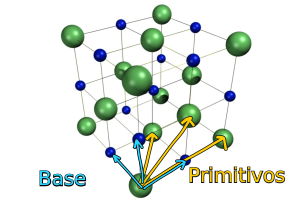
\includegraphics[width=0.5\linewidth,height=0.3\linewidth]{nacl.png}
  \caption{Cloruro de Sodio como dos FCC intercaladas.}
  \label{fig:nacl}
\end{figure}


Vectores primitivos:

$$\begin{cases}
\vec{a}_{1} = a\hat{x} \\
\vec{a}_{2} = \frac{a}{\sqrt{2}}(\hat{x} + \hat{y}) \\
\vec{a}_{3} = \frac{a}{\sqrt{2}}(\hat{x} + \hat{z})
\end{cases}$$

Base:

$$\{\vec{0}, \frac{a}{2}(\hat{x} + \hat{y} + \hat{z}) \}$$

\item Para el Cloruro de Cesio (CsCl), tenemos:

\begin{figure}[H]
  \centering
  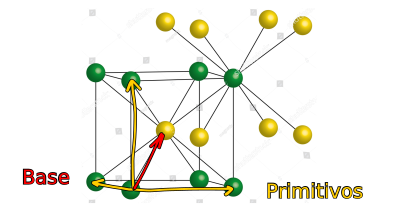
\includegraphics[width=0.5\linewidth,height=0.3\linewidth]{cscl.png}
  \caption{Cloruro de Cesio como dos SC intercaladas.}
  \label{fig:cscl}
\end{figure}

Vectores primitivos:

$$\begin{cases}
\vec{a}_{1} = a\hat{x} \\
\vec{a}_{2} = a\hat{y} \\
\vec{a}_{3} = a\hat{z}
\end{cases}$$

Base:

$$\{\vec{0}, \frac{a}{2\sqrt{3}}(\hat{x} + \hat{y} + \hat{z}) \}$$ 

\item Por \'ultimo, la zincblenda (ZnS) est\'a conformada por una estructura en diamante:

\begin{figure}[H]
  \centering
  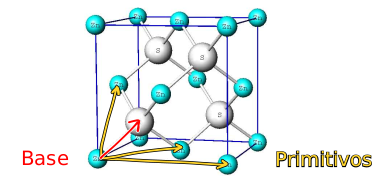
\includegraphics[width=0.5\linewidth,height=0.3\linewidth]{zns.png}
  \caption{Esquema de la zincblenda.}
  \label{fig:zns}
\end{figure}

Vectores primitivos:

$$\begin{cases}
\vec{a}_{1} = \frac{a}{2}(\hat{x} + \hat{y}) \\
\vec{a}_{2} = \frac{a}{2}(\hat{x} + \hat{z}) \\
\vec{a}_{3} = \frac{a}{2}(\hat{y} + \hat{z})
\end{cases}$$

Base:

$$\{\vec{0}, \frac{a}{4}(\hat{x} + \hat{y} + \hat{z}) \}$$ 
\end{itemize}

\subsection{-}
\subsection{-}

\subsection{}

Antes de hacer este ejercicio, repasemos algunas definiciones: \\

La \textbf{red directa} (RD) o red de Bravais se describe como:

\begin{equation}
\label{eq:reddirecta}
\vec{R} = n_{1}\vec{a}_{1} + n_{2}\vec{a}_{2} + n_{3}\vec{a}_{3}
\end{equation}

donde $n_{i} \in \mathbb{Z}$ y $\vec{a}_{i}$ son los vectores primitivos.\\

Por otro lado, la \textbf{red rec\'iproca} (RR) se describe como los vectores $\vec{K}$ que cumplen la relaci\'on:

\begin{equation}
\label{eq:ekr}
e^{\vec{K} \cdot \vec{R}} = 1
\end{equation}

donde $\vec{R}$ es la red de Bravais correspondiente. Una manera m\'as sencilla de definirlos es la siguiente:

\begin{equation}
\label{eq:redreciproca}
\vec{K} = l_{1}\vec{b}_{1} + l_{2}\vec{b}_{2} + l_{3}\vec{b}_{3}
\end{equation}

Nuevamente, $l_{i} \in \mathbb{Z}$ y para $\vec{b}_{i}$ se utiliza esta definici\'on:

$$\vec{b}_{1} = 2\pi  \frac{\vec{a}_{2} \times \vec{a}_{3}}{\vec{a}_{1} \cdot (\vec{a}_{2} \times \vec{a}_{3})}$$

$$\vec{b}_{2} = 2\pi  \frac{\vec{a}_{3} \times \vec{a}_{1}}{\vec{a}_{1} \cdot (\vec{a}_{2} \times \vec{a}_{3})}$$ 

$$\vec{b}_{3} = 2\pi  \frac{\vec{a}_{1} \times \vec{a}_{2}}{\vec{a}_{1} \cdot (\vec{a}_{2} \times \vec{a}_{3})}$$

satisfaciendo que $\vec{b}_{i} \cdot \vec{a}_{j} = 2\pi \delta_{ij}$\\

De acuerdo con la ecuaci\'on (\ref{eq:ekr}), la red rec\'iproca de la red rec\'iproca es un conjunto de todos los vectores $\vec{G}$ que satisfacen:

$$e^{i \vec{G} \cdot \vec{K}} = 1$$

$\forall \vec{K} \in$ RR. Como cualquier vector $\vec{R}$ de la RD tiene esta propiedad (nuevamente, por (\ref{eq:ekr})), todos los vectores de la RD estar\'an en la RR de la RR.\\

\begin{itemize}
\item\textbf{BCC:}

Aplicamos las definiciones para $\vec{b}_{i}$, teniendo en cuenta los vectores primitivos de la red BCC:

$$\begin{cases}
\vec{a}_{1} = a\hat{x} \\
\vec{a}_{2} = \frac{a}{2}(\hat{x} + \hat{y} + \hat{z}) \\
\vec{a}_{3} = a\hat{z}
\end{cases}$$

Sabemos que $V_{BCC} = \vec{a}_{1} \cdot (\vec{a}_{2} \times \vec{a}_{3}) = \frac{a^{3}}{2}$, luego:

$$ \vec{a}_{2} \times \vec{a}_{3} = \begin{vmatrix}
\frac{a}{2} & \frac{a}{2} & \frac{a}{2} \\ 
0 & 0 & a
\end{vmatrix}  = (\frac{a^{2}}{2}, -\frac{a^{2}}{2}, 0) = \frac{a^{2}}{2}(\hat{x} - \hat{y})$$

$$ \vec{a}_{3} \times \vec{a}_{1} = \begin{vmatrix}
0 & 0 & a \\
a & 0 & 0
\end{vmatrix}  = (0, a^{2}, 0) = a^{2}\hat{y}$$

$$ \vec{a}_{1} \times \vec{a}_{2} = \begin{vmatrix}
a & 0 & 0 \\ 
\frac{a}{2} & \frac{a}{2} & \frac{a}{2}
\end{vmatrix}  = (0, -\frac{a^{2}}{2}, \frac{a^{2}}{2}) = \frac{a^{2}}{2}(-\hat{y} + \hat{z})$$

$$\Rightarrow \begin{cases}
\vec{b}_{1} = 2\pi \frac{\frac{a^{2}}{2}(\hat{x} - \hat{y})}{\frac{a^{3}}{2}} = \frac{2\pi}{a}(\hat{x} - \hat{y})\\
\vec{b}_{2} = 2\pi \frac{a^{2}\hat{y}}{\frac{a^{3}}{2}} = \frac{4\pi}{a}\hat{y}\\
\vec{b}_{3} = 2\pi \frac{\frac{a^{2}}{2}(-\hat{y} + \hat{z})}{\frac{a^{3}}{2}} = \frac{2\pi}{a}(-\hat{y} + \hat{z})
\end{cases}$$

Podemos ver que la RR de una BCC es una FCC de lado $\frac{4 \pi}{a}$.

\item\textbf{FCC:}

Vectores primitivos de la red FCC:

$$\begin{cases}
\vec{a}_{1} = \frac{a}{2}(\hat{x} + \hat{y}) \\
\vec{a}_{2} = \frac{a}{2}(\hat{x} + \hat{z}) \\
\vec{a}_{3} = \frac{a}{2}(\hat{y} + \hat{z})
\end{cases}$$

Sabemos que $V_{FCC} = \vec{a}_{1} \cdot (\vec{a}_{2} \times \vec{a}_{3}) = \frac{a^{3}}{4}$, luego:

$$ \vec{a}_{2} \times \vec{a}_{3} = \begin{vmatrix}
\frac{a}{2} & 0 & \frac{a}{2} \\ 
0 & \frac{a}{2} & \frac{a}{2}
\end{vmatrix}  = (-\frac{a^{2}}{4}, -\frac{a^{2}}{4}, \frac{a^{2}}{4}) = \frac{a^{2}}{4}(-\hat{x} - \hat{y} + \hat{z})$$

$$ \vec{a}_{3} \times \vec{a}_{1} = \begin{vmatrix}
0 & \frac{a}{2} & \frac{a}{2} \\
\frac{a}{2} & \frac{a}{2} & 0
\end{vmatrix}  = (-\frac{a^{2}}{4}, \frac{a^{2}}{4}, -\frac{a^{2}}{4}) = \frac{a^{2}}{4}(-\hat{x} + \hat{y} - \hat{z})$$

$$ \vec{a}_{1} \times \vec{a}_{2} = \begin{vmatrix}
\frac{a}{2} & \frac{a}{2} & 0 \\ 
\frac{a}{2} & 0 & \frac{a}{2}
\end{vmatrix}  = (\frac{a^{2}}{4}, -\frac{a^{2}}{4}, -\frac{a^{2}}{4}) = \frac{a^{2}}{4}(\hat{x} - \hat{y} - \hat{z})$$

$$\Rightarrow \begin{cases}
\vec{b}_{1} = 2\pi \frac{\frac{a^{2}}{4}(-\hat{x} - \hat{y} + \hat{z})}{\frac{a^{3}}{4}} = \frac{2\pi}{a}(-\hat{x} - \hat{y} + \hat{z})\\
\vec{b}_{2} = 2\pi \frac{\frac{a^{2}}{4}(-\hat{x} + \hat{y} - \hat{z})}{\frac{a^{3}}{4}} = \frac{2\pi}{a}(-\hat{x} + \hat{y} - \hat{z})\\
\vec{b}_{3} = 2\pi \frac{\frac{a^{2}}{4}(\hat{x} - \hat{y} - \hat{z})}{\frac{a^{3}}{4}} = \frac{2\pi}{a}(\hat{x} - \hat{y} - \hat{z})
\end{cases}$$

Vemos que la RR de una FCC es una BCC de lado $\frac{4 \pi}{a}$ (pues $\frac{2 \pi}{a} = \frac{4 \pi}{a}\frac{1}{2}$).

\end{itemize}

Algunos ejemplos de redes autorrec\'iprocas (RD = RR) son la SC y la hexagonal simple, a menos de las constantes de red.

\subsection{}

Para ver las zonas de Brillouin (ZB), primero calculemos la RR de la SC en dos dimensiones:

$$\begin{cases}
\vec{a}_{1} = a\hat{x} \\
\vec{a}_{2} = a\hat{y}
\end{cases}$$

$$\Rightarrow \begin{cases}
\vec{b}_{1} = \frac{2 \pi}{a}\hat{x} \\
\vec{b}_{2} = \frac{2 \pi}{a}\hat{y}
\end{cases}$$

A continuaci\'on, se detallan a modo de receta los pasos para dibujar las primeras ZB de la red:

\begin{itemize}
\item Identificar los primeros vecinos en la RR y dibujar una linea perpendicular (plano de Bragg) atravesando el punto medio entre el \'atomo de referencia y cada uno de sus vecinos. Luego, el \'area roja que encierra al origen entre los planos de Bragg es la \textbf{primera zona de Brillouin (1ZB) o celda de Wigner-Seitz}:

\begin{figure}[H]
  \centering
  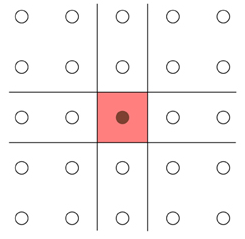
\includegraphics[width=0.3\linewidth,height=0.3\linewidth]{pzb.png}
  \caption{Construcci\'on de la 1ZB para la red SC.}
  \label{fig:pzb}
\end{figure}

\item La \textbf{segunda zona de Brillouin (2ZB)} es el espacio de la RR en el cual un punto tiene un plano de Bragg entre \'este y el origen. Como muestra la siguiente figura, trazamos los planos de Bragg correspondientes a los segundos vecinos y marcamos el \'area en amarillo:

\begin{figure}[H]
  \centering
  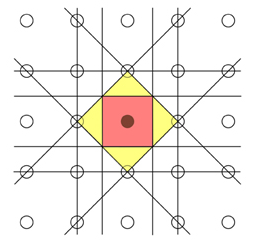
\includegraphics[width=0.3\linewidth,height=0.3\linewidth]{szb.png}
  \caption{Construcci\'on de la 2ZB para la red SC. Notar los planos de Bragg entre los segundos vecinos y el origen (mostrados en la figura (\ref{fig:pzb})), para poder identificar correctamente la zona.}
  \label{fig:szb}
\end{figure}

\end{itemize}

Sistem\'aticamente, se construyen as\'i las siguientes zonas de Brillouin, tomando los terceros vecinos, etc. En el siguiente esquema se muestran las tres primeras ZB para la red SC:

\begin{figure}[H]
  \centering
  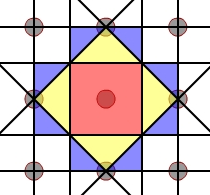
\includegraphics[width=0.3\linewidth,height=0.3\linewidth]{zb.png}
  \caption{1ZB (rojo), 2ZB (amarillo) y 3ZB (violeta) de la red SC bidimensional.}
  \label{fig:zb}
\end{figure}

Los volumenes de cada zona ser\'an los mismos, debido a que la RR es peri\'odica, para un punto fuera de la 1ZB existe un \'unico vector de la RR que lo traslade nuevamente hacia la primera zona, por lo tanto todas las zonas tienen el mismo \'area o volumen.\\

En nuestro caso, $V_{1ZB} = (\frac{2 \pi}{a})^{2} = \frac{4 \pi^{2}}{a^{2}} = V_{2ZB} = V_{3ZB}$

\subsection{}

\begin{itemize}
\item Vectores primitivos de la red hexagonal:

$$\begin{cases}
\vec{a}_{1} = - \frac{\sqrt{3}}{2}a\hat{x} + \frac{a}{2}\hat{y} \\
\vec{a}_{2} = - \frac{\sqrt{3}}{2}a\hat{x} + \frac{a}{2}\hat{y} \\
\vec{a}_{3} = c\hat{z}
\end{cases}$$

$$\Rightarrow V_{Hexagonal} = | \vec{a}_{1} \cdot (\vec{a}_{2} \times \vec{a}_{3})| = \frac{\sqrt{3}}{2}a^{2}c$$

\item Vectores de la red rec\'iproca (ver ejercicio 9 para el procedimiento general en detalle):

$$\begin{cases}
\vec{b}_{1} = \frac{2 \pi}{\sqrt{3}a}\hat{x} + \frac{2 \pi}{a}\hat{y} \\
\vec{b}_{2} = - \frac{2 \pi}{\sqrt{3}a}\hat{x} + \frac{2 \pi}{a}\hat{y} \\
\vec{b}_{3} = \frac{2 \pi}{c}\hat{z}
\end{cases}$$

\item Esquema y descripci\'on de la primera zona de Brillouin de la red hexagonal:

\begin{figure}[H]
  \centering
  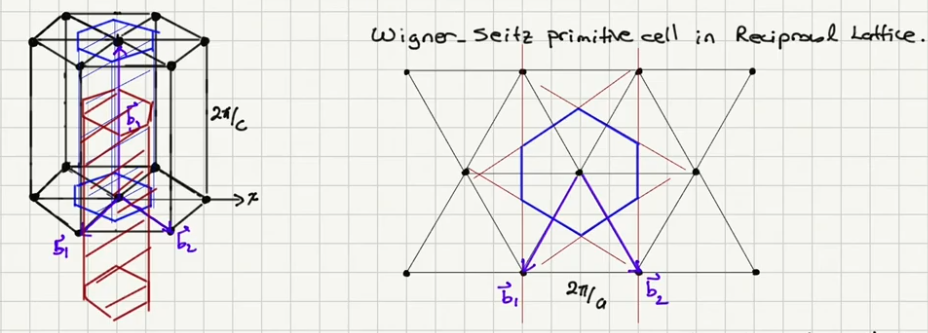
\includegraphics[width=0.9\linewidth,height=0.5\linewidth]{pzb_hex.png}
  \caption{Las bisectrices en los puntos medios de $\vec{b}_{1}$, -$\vec{b}_{1}$, $\vec{b}_{2}$, -$\vec{b}_{2}$, $\vec{b}_{1} - \vec{b}_{2}$ y $\vec{b}_{2} - \vec{b}_{1}$ forman un hex\'agono (mostrados en detalle en la celda de Wigner-Seitz). La 1ZB (prisma sombreado en color rojo) estar\'a dada por \'este hex\'agono y la bisectriz en el punto medio entre $\vec{b}_{3}$ y $-\vec{b}_{3}$.}
  \label{fig:pzb_hex}
\end{figure}

\end{itemize}

\subsection{}

Los \'indices de Miller est\'an dados por los coeficientes $(hkl)$ que acompa\~nan a los $\vec{b}_{i}$ en el vector del espacio rec\'iproco $\vec{K} = h\vec{b}_{1} + k\vec{b}_{2} + l\vec{b}_{3}$. Si alguno de los \'indices es negativo, por ejemplo $h$, se nota como $\overline{h}$.

\begin{itemize}
\item \textbf{Red SC:}

$$\begin{cases}
\vec{b}_{1} = \frac{2 \pi}{a}\hat{x}\\
\vec{b}_{2} = \frac{2 \pi}{a}\hat{y} \\
\vec{b}_{3} = \frac{2 \pi}{a}\hat{z}
\end{cases}$$

$$\Rightarrow \vec{K}_{hkl} = \frac{2 \pi}{a}h\hat{x} + \frac{2 \pi}{a}k\hat{y} + \frac{2 \pi}{a}l\hat{z}$$

Veamos ahora los $\vec{K}$ y la distancia entre planos $d$ para los \'indices pedidos en el enunciado:

$$(100) \rightarrow \vec{K}_{100} = \frac{2 \pi}{a}(1\hat{x} + 0\hat{y} + 0\hat{z}) = \frac{2 \pi}{a}\hat{x}$$

$$(110) \rightarrow \vec{K}_{110} = \frac{2 \pi}{a}(1\hat{x} + 1\hat{y} + 0\hat{z}) = \frac{2 \pi}{a}(\hat{x} + \hat{y})$$

$$(111) \rightarrow \vec{K}_{111} = \frac{2 \pi}{a}(1\hat{x} + 1\hat{y} + 1\hat{z}) = \frac{2 \pi}{a}(\hat{x} + \hat{y} + \hat{z})$$

\begin{figure}[H]
  \centering
  \begin{subfigure}[b]{0.4\linewidth}
    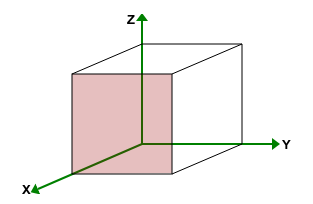
\includegraphics[width=\linewidth]{miller_sc100.png}
     \caption{Plano (100)}
  \end{subfigure}
  \begin{subfigure}[b]{0.4\linewidth}
    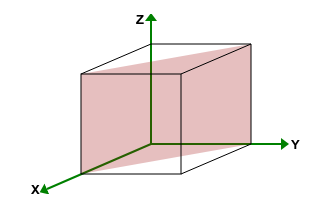
\includegraphics[width=\linewidth]{miller_sc110.png}
    \caption{Plano (110)}
  \end{subfigure}
  \begin{subfigure}[b]{0.4\linewidth}
    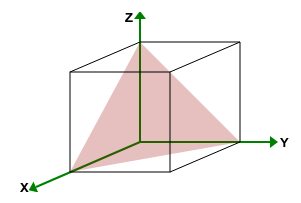
\includegraphics[width=\linewidth]{miller_sc111.png}
    \caption{Plano (111)}
  \end{subfigure}
  \caption{Planos dados por los \'indices de Miller $(hkl)$.}
  \label{fig:miller_planos}
\end{figure}

Distancia entre planos $d = \frac{2\pi}{|\vec{K}|}$:

$$| \vec{K}_{100} | = \sqrt{\bigg(\frac{2 \pi}{a}\bigg)^{2}} =  \frac{2\pi}{d_{100}} \Rightarrow d_{100} = a$$

$$| \vec{K}_{110} | = \sqrt{\bigg(\frac{2 \pi}{a}\bigg)^{2} + \bigg(\frac{2 \pi}{a}\bigg)^{2}} = \sqrt{2} \frac{2\pi}{a} =  \frac{2\pi}{d_{110}} \Rightarrow d_{110} = \frac{a}{\sqrt{2}}$$

$$| \vec{K}_{111} | = \sqrt{\bigg(\frac{2 \pi}{a}\bigg)^{2} + \bigg(\frac{2 \pi}{a}\bigg)^{2} + \bigg(\frac{2 \pi}{a}\bigg)^{2}} = \sqrt{3} \frac{2\pi}{a} =  \frac{2\pi}{d_{111}} \Rightarrow d_{111} = \frac{a}{\sqrt{3}}$$
\\

\item \textbf{Red FCC:}

$$\begin{cases}
\vec{b}_{1} = \frac{2 \pi}{a}(-\hat{x} - \hat{y} + \hat{z})\\
\vec{b}_{2} = \frac{2 \pi}{a}(-\hat{x} + \hat{y} - \hat{z}) \\
\vec{b}_{3} = \frac{2 \pi}{a}(\hat{x} - \hat{y} - \hat{z})
\end{cases}$$

$$\Rightarrow \vec{K}_{hkl} = \frac{2 \pi}{a}h(-\hat{x} - \hat{y} + \hat{z}) + \frac{2 \pi}{a}k(-\hat{x} + \hat{y} - \hat{z}) + \frac{2 \pi}{a}l(\hat{x} - \hat{y} - \hat{z})$$



$$(100) \rightarrow \vec{K}_{100} = \frac{2 \pi}{a}(-\hat{x} - \hat{y} + \hat{z})$$

$$(110) \rightarrow \vec{K}_{110} = \frac{2 \pi}{a}(-\hat{x} - \hat{y} + \hat{z} -\hat{x} + \hat{y} - \hat{z}) = -\frac{4 \pi}{a}\hat{x}$$

$$(111) \rightarrow \vec{K}_{111} = \frac{2 \pi}{a}(-\hat{x} - \hat{y} + \hat{z} -\hat{x} + \hat{y} - \hat{z} + \hat{x} - \hat{y} - \hat{z}) = \frac{2 \pi}{a}(-\hat{x} - \hat{y} - \hat{z})$$


Distancia entre planos $d = \frac{2\pi}{|\vec{K}|}$:

$$| \vec{K}_{100} | = \sqrt{\bigg(-\frac{2 \pi}{a}\bigg)^{2} + \bigg(-\frac{-2 \pi}{a}\bigg)^{2} + \bigg(\frac{2 \pi}{a}\bigg)^{2}} =  \sqrt{3} \frac{2\pi}{a} =  \frac{2\pi}{d_{100}} \Rightarrow d_{100} = \frac{a}{\sqrt{3}}$$

$$| \vec{K}_{110} | = \sqrt{\bigg(-\frac{4 \pi}{a}\bigg)^{2}} = \frac{4\pi}{a} =  \frac{2\pi}{d_{110}} \Rightarrow d_{110} = \frac{a}{2}$$

$$| \vec{K}_{111} | = | \vec{K}_{100} | \Rightarrow d_{111} = \frac{a}{\sqrt{3}}$$
\\

\item \textbf{Red BCC:}

$$\begin{cases}
\vec{b}_{1} = \frac{2 \pi}{a}(\hat{x} - \hat{y})\\
\vec{b}_{2} = \frac{4 \pi}{a}\hat{y}\\
\vec{b}_{3} = \frac{2 \pi}{a}(- \hat{y} + \hat{z})
\end{cases}$$

$$\Rightarrow \vec{K}_{hkl} = \frac{2 \pi}{a}h(\hat{x} - \hat{y}) + \frac{4 \pi}{a}k\hat{y} + \frac{2 \pi}{a}l(-\hat{y} + \hat{z})$$



$$(100) \rightarrow \vec{K}_{100} = \frac{2 \pi}{a}(\hat{x} - \hat{y})$$

$$(110) \rightarrow \vec{K}_{110} = \frac{2 \pi}{a}(\hat{x} - \hat{y} + 2\hat{y}) = \frac{2 \pi}{a}(\hat{x} + \hat{y})$$

$$(111) \rightarrow \vec{K}_{111} = \frac{2 \pi}{a}(\hat{x} - \hat{y} + 2\hat{y} - \hat{y} + \hat{z}) = \frac{2 \pi}{a}(\hat{x} + \hat{z})$$


Distancia entre planos $d = \frac{2\pi}{|\vec{K}|}$:

$$| \vec{K}_{100} | = \sqrt{\bigg(\frac{2 \pi}{a}\bigg)^{2} + \bigg(-\frac{2 \pi}{a}\bigg)^{2}} =  \sqrt{2} \frac{2\pi}{a} =  \frac{2\pi}{d_{100}} \Rightarrow d_{100} = \frac{a}{\sqrt{2}}$$

$$| \vec{K}_{110} | =  \sqrt{\bigg(\frac{2 \pi}{a}\bigg)^{2} + \bigg(\frac{2 \pi}{a}\bigg)^{2}} =  \sqrt{2} \frac{2\pi}{a} =  \frac{2\pi}{d_{110}} \Rightarrow d_{110} = \frac{a}{\sqrt{2}}$$

$$| \vec{K}_{111} | = | \vec{K}_{110} | \Rightarrow d_{111} = \frac{a}{\sqrt{2}}$$

\end{itemize}

\subsection{}

Celda convencional ortorr\'ombica ($a = 2 \r{A}$, $b = 3 \r{A}$, $c = 4 \r{A}$; $\alpha = \beta = \gamma = \frac{\pi}{2}$):

\begin{figure}[H]
  \centering
  \begin{subfigure}[b]{0.4\linewidth}
    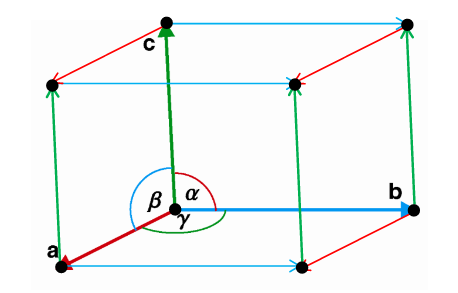
\includegraphics[width=\linewidth]{tetragonal.png}
     \caption{Cristal con par\'ametros de red y \'angulos generales.}
  \end{subfigure}
  \begin{subfigure}[b]{0.35\linewidth}
    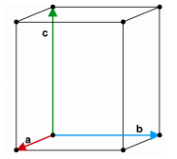
\includegraphics[width=\linewidth]{ortorrombico.png}
    \caption{Cristal ortorr\'ombico.}
  \end{subfigure}
  \caption{Esquema y caso particular de estructuras cristalinas.}
  \label{fig:ortorrombico}
\end{figure}

$$\begin{cases}
\vec{a}_{1} = 2 \textup{\r{A}}\hat{x}\\
\vec{a}_{2} = 3 \textup{\r{A}} \hat{y} \\
\vec{a}_{3} = 4 \textup{\r{A}} \hat{z}
\end{cases}$$

$$\Rightarrow V_{O} = | \vec{a}_{1} \cdot (\vec{a}_{2} \times \vec{a}_{3})| = 24 \textup{\r{A}}^{3} $$

$$\Rightarrow \begin{cases}
\vec{b}_{1} = \frac{\pi}{\textup{\r{A}}}\hat{x} \\
\vec{b}_{2} = \frac{2\pi}{3\textup{\r{A}}}\hat{y} \\
\vec{b}_{3} = \frac{\pi}{2\textup{\r{A}}}\hat{z}
\end{cases}$$

$$\Rightarrow \vec{K}_{112} = 1\vec{b}_{1} + 1\vec{b}_{2} + 2\vec{b}_{3} = \frac{\pi}{\textup{\r{A}}}\hat{x} + \frac{2\pi}{3\textup{\r{A}}}\hat{y} + \frac{\pi}{\textup{\r{A}}}\hat{z}$$

Luego

$$| \vec{K}_{112} | = \sqrt{\bigg(\frac{\pi}{\textup{\r{A}}}\bigg)^{2} + \bigg(\frac{2\pi}{3\textup{\r{A}}}\bigg)^{2} + \bigg(\frac{\pi}{\textup{\r{A}}}\bigg)^{2}} =  \sqrt{\frac{22}{3}} \frac{\pi}{\textup{\r{A}}} =  \frac{2\pi}{d_{112}}$$

$$ \Rightarrow d_{112} = \sqrt{\frac{6}{11}}\textup{\r{A}} \approx 0.74 \textup{\r{A}}$$

\subsection{}

Veamos primero $\vec{K}_{100}$ y $\vec{K}_{001}$ para los siguientes vectores primitivos:

$$\begin{cases}
\vec{a}_{1} = \frac{a}{2} (\hat{y} + \hat{z})\\
\vec{a}_{2} = \frac{a}{2} (\hat{x} + \hat{z}) \\
\vec{a}_{3} = \frac{a}{2} (\hat{x} + \hat{y})
\end{cases}$$

$$\Rightarrow V_{FCC} = | \vec{a}_{1} \cdot (\vec{a}_{2} \times \vec{a}_{3})| = \frac{a^{3}}{4} $$

$$\Rightarrow \begin{cases}
\vec{b}_{1} = \frac{2\pi}{a}(-\hat{x} + \hat{y} + \hat{z}) \\
\vec{b}_{2} = \frac{2\pi}{a}(\hat{x} - \hat{y} + \hat{z}) \\
\vec{b}_{3} = \frac{2\pi}{a}(\hat{x} + \hat{y} - \hat{z})
\end{cases}$$

Luego, $\vec{K}_{hkl} = h\vec{b}_{1} + k\vec{b}_{2} + l\vec{b}_{3} = h\frac{2\pi}{a}(-\hat{x} + \hat{y} + \hat{z}) + k\frac{2\pi}{a}(\hat{x} - \hat{y} + \hat{z}) + l\frac{2\pi}{a}(\hat{x} + \hat{y} - \hat{z})$

$$\Rightarrow \begin{cases}
\vec{K}_{100} = \frac{2\pi}{a}(-\hat{x} + \hat{y} + \hat{z}) \\
\vec{K}_{001} = \frac{2\pi}{a}(\hat{x} + \hat{y} - \hat{z}) 
\end{cases}$$
\\

Ahora, calculemos los \'indices de Miller para los $\vec{a}_{i}'$ definidos en el enunciado:

$$\begin{cases}
\vec{a}_{1}' = a\hat{x}\\
\vec{a}_{2}' = \frac{a}{2} (\hat{x} + \hat{y}) \\
\vec{a}_{3}' = \frac{a}{2} (\hat{y} + \hat{z})
\end{cases}$$

$$\Rightarrow V_{FCC} = | \vec{a}_{1}' \cdot (\vec{a}_{2}' \times \vec{a}_{3}')| = \frac{a^{3}}{4} $$

$$\Rightarrow \begin{cases}
\vec{b}_{1}' = \frac{2\pi}{a}(\hat{x} - \hat{y} + \hat{z}) \\
\vec{b}_{2}' = \frac{4\pi}{a}(\hat{y} + \hat{z}) \\
\vec{b}_{3}' = \frac{4\pi}{a}\hat{z}
\end{cases}$$

Entonces, $\vec{K}_{h'k'l'}' = h'\vec{b}_{1}' + k'\vec{b}_{2}' + l'\vec{b}_{3}' = h'\frac{2\pi}{a}(\hat{x} - \hat{y} + \hat{z}) + k'\frac{4\pi}{a}(\hat{y} + \hat{z}) + l'\frac{4\pi}{a}\hat{z}$
\\

Finalmente, comparamos en cada direcci\'on los $\vec{K}_{hkl}$ y $\vec{K'}_{h'k'l'}$:

\begin{itemize}
\item $\vec{K}_{100}$:

$$ \hat{x}) h'\frac{2\pi}{a} = -\frac{2\pi}{a} \Rightarrow h' = -1$$
$$ \hat{y}) h'\frac{2\pi}{a} + k'\frac{4\pi}{a} = \frac{2\pi}{a} \Rightarrow k' = 0$$
$$ \hat{z}) h'\frac{2\pi}{a} - k'\frac{4\pi}{a} + l'\frac{4\pi}{a} = \frac{2\pi}{a} \Rightarrow l' = 1$$

Por lo tanto, $(100)$ corresponden a $(\overline{1}01)$.


\item $\vec{K}_{001}$:

$$ \hat{x}) h'\frac{2\pi}{a} = \frac{2\pi}{a} \Rightarrow h' = 1$$
$$ \hat{y}) -h'\frac{2\pi}{a} + k'\frac{4\pi}{a} = \frac{2\pi}{a} \Rightarrow k' = 1$$
$$ \hat{z}) h'\frac{2\pi}{a} - k'\frac{4\pi}{a} + l'\frac{4\pi}{a} = -\frac{2\pi}{a} \Rightarrow l' = 0$$

Entonces, $(001)$ corresponden a $(110)$.

\end{itemize}

\subsection{}

El factor de estructura se define como:

\begin{equation}
\label{eq:fe}
S_{\vec{K}} = \sum_{j} f_{j}(\vec{K})e^{i\vec{K} \cdot \vec{d}_{j}}
\end{equation}

donde $\vec{K} \in$ RR, y $\vec{d}_{j}$ es el $j$-\'esimo vector de la base de la red.\\

Escribimos a la red FCC como SC + $\{{\vec{0}, \frac{a}{2}(\hat{x} + \hat{y}), \frac{a}{2}(\hat{x} + \hat{z}), \frac{a}{2}(\hat{y} + \hat{z})}\}$. Reemplazando esto en la ecuaci\'on (\ref{eq:fe}) teniendo en cuenta que los $f_{j}(\vec{K})$ son todos iguales (mismo tipo de \'atomo en toda la red) y adem\'as $\vec{K} = \frac{2\pi}{a}(n_{1}\hat{x} + n_{2}\hat{y} + n_{3}\hat{z})$, obtenemos:

$$S_{\vec{K}} = \sum_{j = 1}^{4} fe^{i\vec{K} \cdot \vec{d}_{j}} = f\sum_{j = 1}^{4} e^{i\vec{K} \cdot \vec{d}_{j}} = f\bigg(1 + e^{i\vec{K} \cdot \frac{a}{2}(\hat{x} + \hat{y})} + e^{i\vec{K} \cdot \frac{a}{2}(\hat{x} + \hat{z})} + e^{i\vec{K} \cdot \frac{a}{2}(\hat{y} + \hat{z})}\bigg)$$

$$\Rightarrow S_{\vec{K}} = f\bigg(1 + e^{i\pi(n_{2} + n_{3})} + e^{i\pi(n_{1} + n_{3})} + e^{i\pi(n_{1} + n_{2})}\bigg) = f\bigg(1 + (-1)^{n_{2} + n_{3}} + (-1)^{n_{1} + n_{3}} + (-1)^{n_{1} + n_{2}}\bigg)$$
\\

En conclusi\'on, $S_{\vec{K}} = 4f$ si los $n_{i}$ son todos pares o impares. En cualquier otro caso, $S_{\vec{K}} = 0$.\\

Si tomamos $f = 1$, obtenemos el resultado del enunciado.\\

Si se remueven los puntos tales que $S_{\vec{K}} = 0$, nos queda una red BCC de par\'ametro $\frac{4\pi}{a}$, ya que es la RR de una FCC con par\'ametro $a$.

\begin{figure}[H]
  \centering
  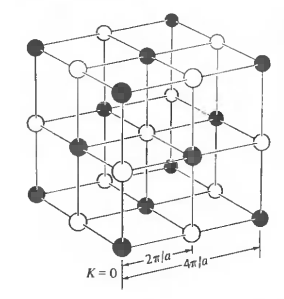
\includegraphics[width=0.3\linewidth,height=0.3\linewidth]{sk.png}
  \caption{Los puntos en negro son los que cumplen que $S_{\vec{K}} = 0$ (alg\'un $n_{i}$ par y los dem\'as pares, o viceversa), por lo tanto se remueven de la red; quedando solo los puntos en blanco (todos los $n_{i}$ con la misma paridad) conformando una BCC.}
  \label{fig:sk}
\end{figure}

\subsection{}
\subsection{}

Si asumimos que los iones de la base no son id\'enticos, el factor de estructura est\'a dado por la forma general vista en la ecuaci\'on (\ref{eq:fe}), donde $f_{j}(\vec{K})$ est\'a completamente determinado por la estructura interna del i\'on en la posici\'on $d_{j}$ de la base.\\

Dicho valor $f_{j}(\vec{K})$ es proporcional a la transformada de Fourier de la distribuci\'on de carga del i\'on correspondiente, es decir:

\begin{equation}
\label{eq:fk}
f_{j}(\vec{K}) = -\frac{1}{e}\int d\vec{r} e^{i\vec{K} \cdot \vec{r}} \rho_{j}(\vec{r}) 
\end{equation}

Ahora bien, el enunciado nos dice que, a su vez, el i\'on $i$-\'esimo est\'a formado por $m_{i}$ part\'iculas puntuales de carga $-z_{ij}e$, localizadas en posiciones $\vec{b}_{ij}$, por lo tanto la ecuaci\'on (\ref{eq:fk}) para cada i\'on se transforma en la siguiente suma discreta:

\begin{equation}
\label{eq:fi}
f_{i}(\vec{K}) = -\frac{1}{e}\sum_{j = 1}^{m_{j}}e^{i\vec{K} \cdot \vec{b}_{ij}}(-z_{ij}e) = \sum_{j = 1}^{m_{j}}z_{ij}e^{i\vec{K} \cdot \vec{b}_{ij}}
\end{equation}
\\

$$\Rightarrow S_{\vec{K}} = \sum_{j = 1}^{n} f_{j}(\vec{K})e^{i\vec{K} \cdot \vec{d}_{j}} = \sum_{j = 1}^{n} \bigg(\sum_{l = 1}^{m_{l}}z_{jl}e^{i\vec{K} \cdot \vec{b}_{jl}}\bigg)e^{i\vec{K} \cdot \vec{d}_{j}} =  \sum_{j = 1}^{n}\sum_{l = 1}^{m_{l}}z_{jl}e^{i\vec{K} \cdot (\vec{b}_{jl} + \vec{d}_{j})}$$ 
\\
\textit{Nota: Creo que por este camino llego a algo parecido a lo que pide el enunciado, hay que jugar un poco con los \'indices y tratar de llevarlo a la forma de la ecuaci\'on (\ref{eq:fe}).}


\begin{center}
\noindent\rule{15cm}{0.4pt}
\end{center}

\section{Gu\'ia 2: Energ\'ia de cohesi\'on}

\subsection{}

%----------------------------------------------------------------------------------------
%	REFERENCE LIST
%----------------------------------------------------------------------------------------
\newpage
\begin{thebibliography}{99} % Bibliography - this is intentionally simple in this template
 
\end{thebibliography}


%----------------------------------------------------------------------------------------

\end{document}